\chapter{Methods} \label{sec:methods}

The primary goal of this study is to assess the practical utility of synthetic images produced by text-to-image models in real-world computer vision tasks. Consequently, the key contribution of this research involves developing a pipeline capable of incorporating synthetic images into the training process of deep learning models. Furthermore, this paper incorporates comprehensive experimentation to demonstrate the efficacy of this approach.

The constructed pipeline addresses the necessity of implementing the innovative task of \textit{generative data augmentation}. The underlying concept of this approach involves utilising generative models to produce synthetic data to augment deep learning datasets. At the time of writing, there are no implementations for this novel data augmentation technique in the leading deep learning libraries. Consequently, we have opted to develop the pipeline from its foundational components. Figure \ref{fig:genaug} shows a schema of the generative augmentation approach.

\begin{figure}
    \centering
    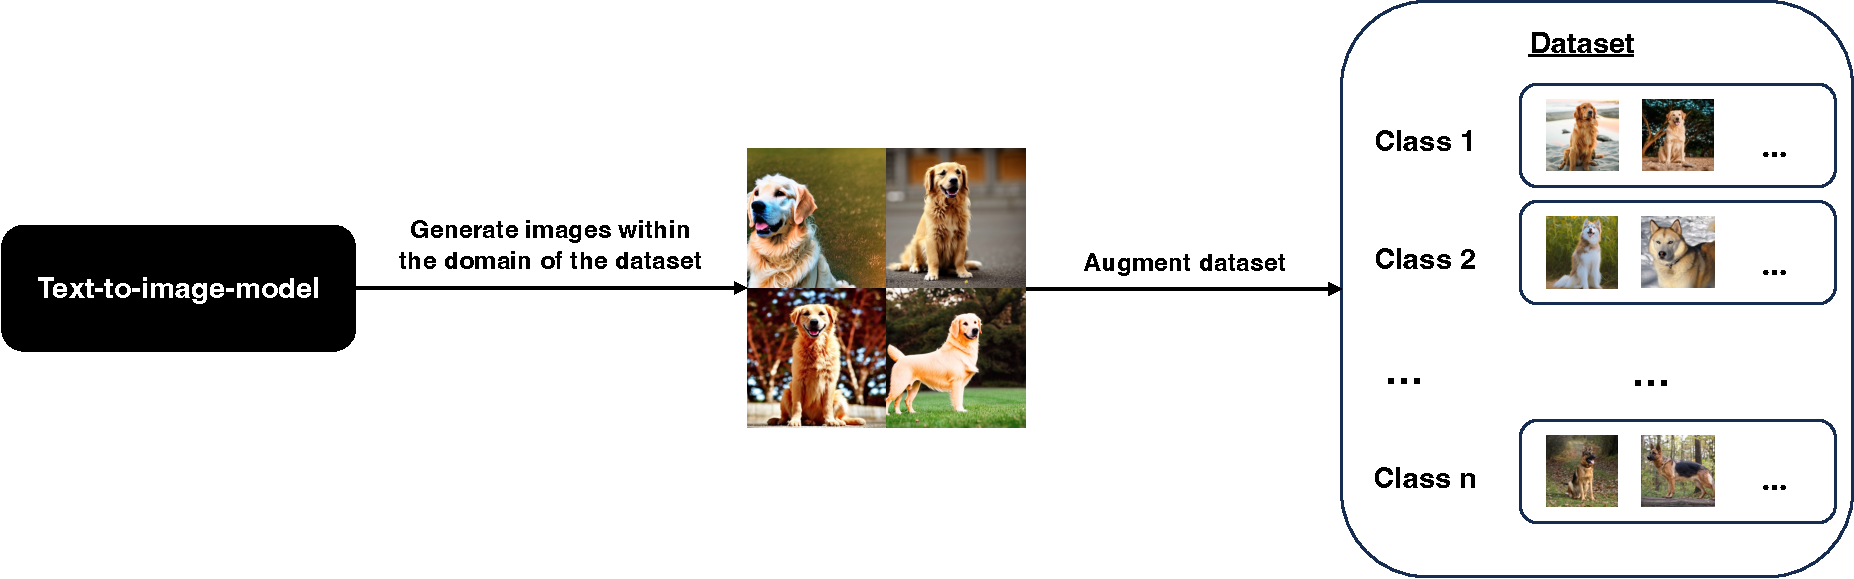
\includegraphics[width=1\textwidth]{Pictures/generative-augmentation.pdf}
    \caption{\textbf{Generative data augmentation}. The concept involves utilizing a text-to-image model to produce synthetic images. These images serve the purpose of augmenting a dataset.}
    \label{fig:genaug}
\end{figure}

\section{Subject-driven augmentation} \label{sec: sdAugmentation}

One of the most promising subfields within \textit{generative augmentation} is \textit{subject-driven augmentation}. This approach synthesises new representations of a specific subject in different contexts. To achieve this, it has to maintain high fidelity to its key visual features. Therefore, we employ the two most relevant techniques within this subfield in our pipeline, Dreambooth and Textual inversion.

Given a dataset categorised into classes, a specific one is taken for analysis. Subsequently, we randomly select 3 to 5 images from this class. The subject-driven technique then modifies a text-to-image model, enabling it to generate synthetic images specific to the chosen subject or class. By adding these images to the training set of a successive task, the original images are automatically augmented. Figure \ref{fig:sdaug} shows a schematic of this subject-driven approach.

\begin{figure}
    \centering
    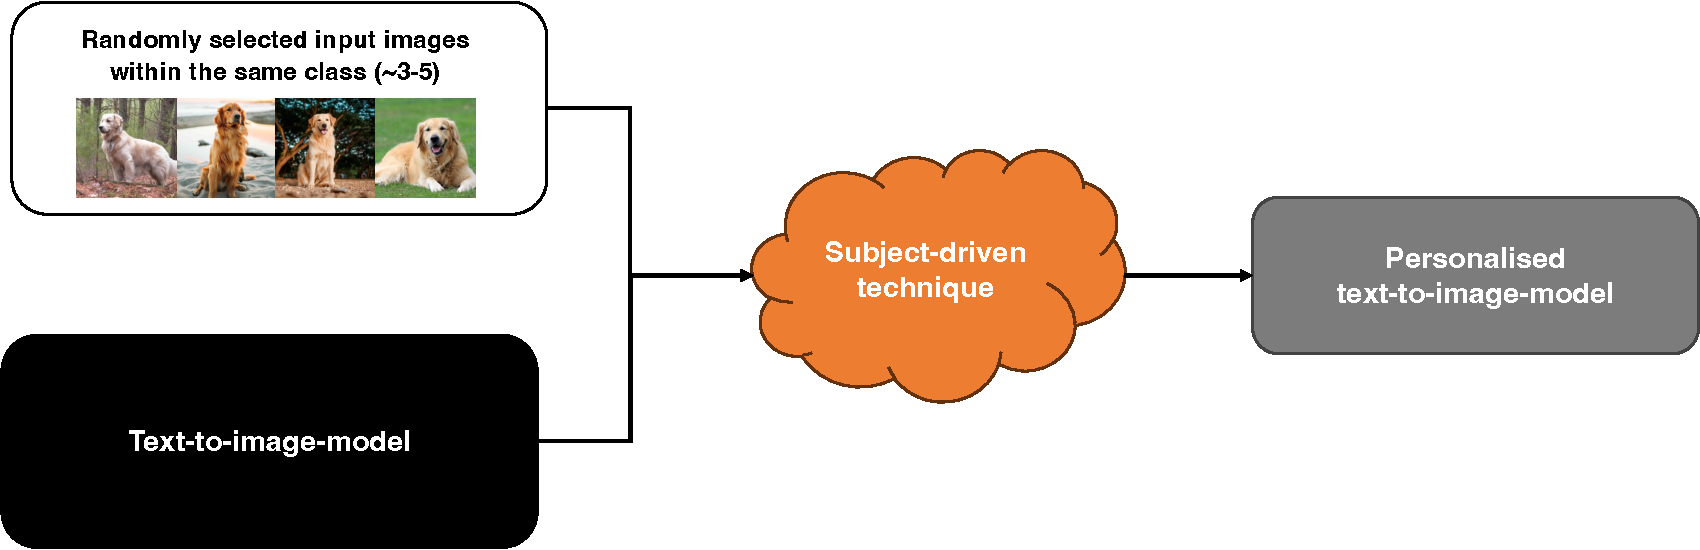
\includegraphics[width=1\textwidth]{Pictures/subject-driven-augmentation.pdf}
    \caption{\textbf{Subject-driven augmentation}. The objective is to personalise a text-to-image model to generate synthetic images of a subject of the class under consideration in novel contexts. To achieve this, multiple images (~3-5) from the class are employed  alongside one of the subject-driven techniques discussed (Dreambooth or Textual inversion).}
    \label{fig:sdaug}
\end{figure}

\section{Class-name-based augmentation} \label{sec: cnbAugmentation}

Both Dreambooth and Textual inversion strategies allow the developed pipeline to be generalist and suitable to be applied in a wide range of scenarios. However, it is a complex approach that requires customising a text-to-image model for each of the classes contained in the considered dataset. Dreambooth requires fine-tuning of the model, whereas, in Textual inversion, the embedding token must be found for a new token corresponding to the considered subject. Consequently, if the aim is to augment a dataset containing numerous diverse classes, a considerable amount of time will be required. Therefore, we propose a solution using the image generation model directly. For this purpose, we solely use the names of the classes used to build the dataset. We build a prompt with it and directly generate images of the targeted class.

This approach resolves the challenge of customising the text-to-image model, consequently reducing the time required for data augmentation. However, employing solely the class name introduces a fundamental issue. The image generation model may not have enough information to be able to generalise images of certain classes. This will, of course, depend on how sparse the presence of objects of the class is in the training set of images of the text-to-image model. Consequently, there will be no complications for classes representing common objects that have extensively contributed to the model's training. Conversely, when operating in a non-common domain, the quality of images generated through this approach may not meet the standards required for inclusion in the augmented dataset. Figure \ref{fig:classaug} shows an outline of the pipeline considering only the class name when generating the synthetic images.

\begin{figure}
    \centering
    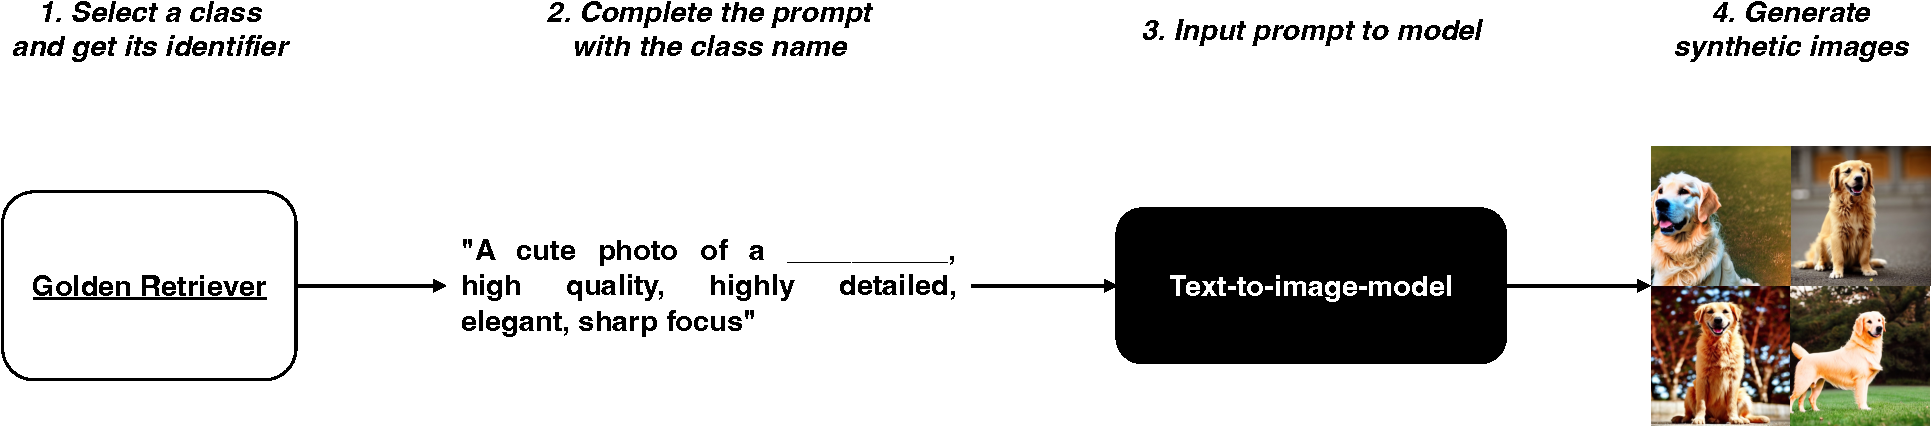
\includegraphics[width=1\textwidth]{Pictures/class-name-augmentation.pdf}
    \caption{\textbf{Class-name-based augmentation}. The difference with the subject-driven schema is that the image generation model is used directly. Only the names of the classes used to build the dataset are employed to generate the synthetic images. With the class name, a suitable and general prompt is generated.}
    \label{fig:classaug}
\end{figure}


\section{Conditionally controlled augmentation} \label{sec: ccAugmentation}

The subject-driven and the class-name-based approaches have straightforward applications in tasks such as classification. However, a challenge arises when aiming to control the generated images for tasks like segmentation. Specifically, generating subjects with specific poses or arrangements becomes difficult due to limitations in textual descriptions' ability to convey precise visual details. We propose integrating ControlNet into the pipeline to introduce conditional control to address this challenge. Taking the pipeline for the class-name-based augmentation case, the only thing that needs to be added is conditional control for the text-to-image model. In this way, a control element must be provided for each image to be generated. As we consider a segmentation task, segmentation maps can be provided, although other alternatives, such as Canny edge detections, may also be valid. With this modification, the generated image will have the layout of the provided condition. Therefore, the image can be used with its associated segmentation map to augment the datasets used in segmentation tasks. Figure \ref{fig:condaug} provides a visual representation of this strategy.

\begin{figure}
    \centering
    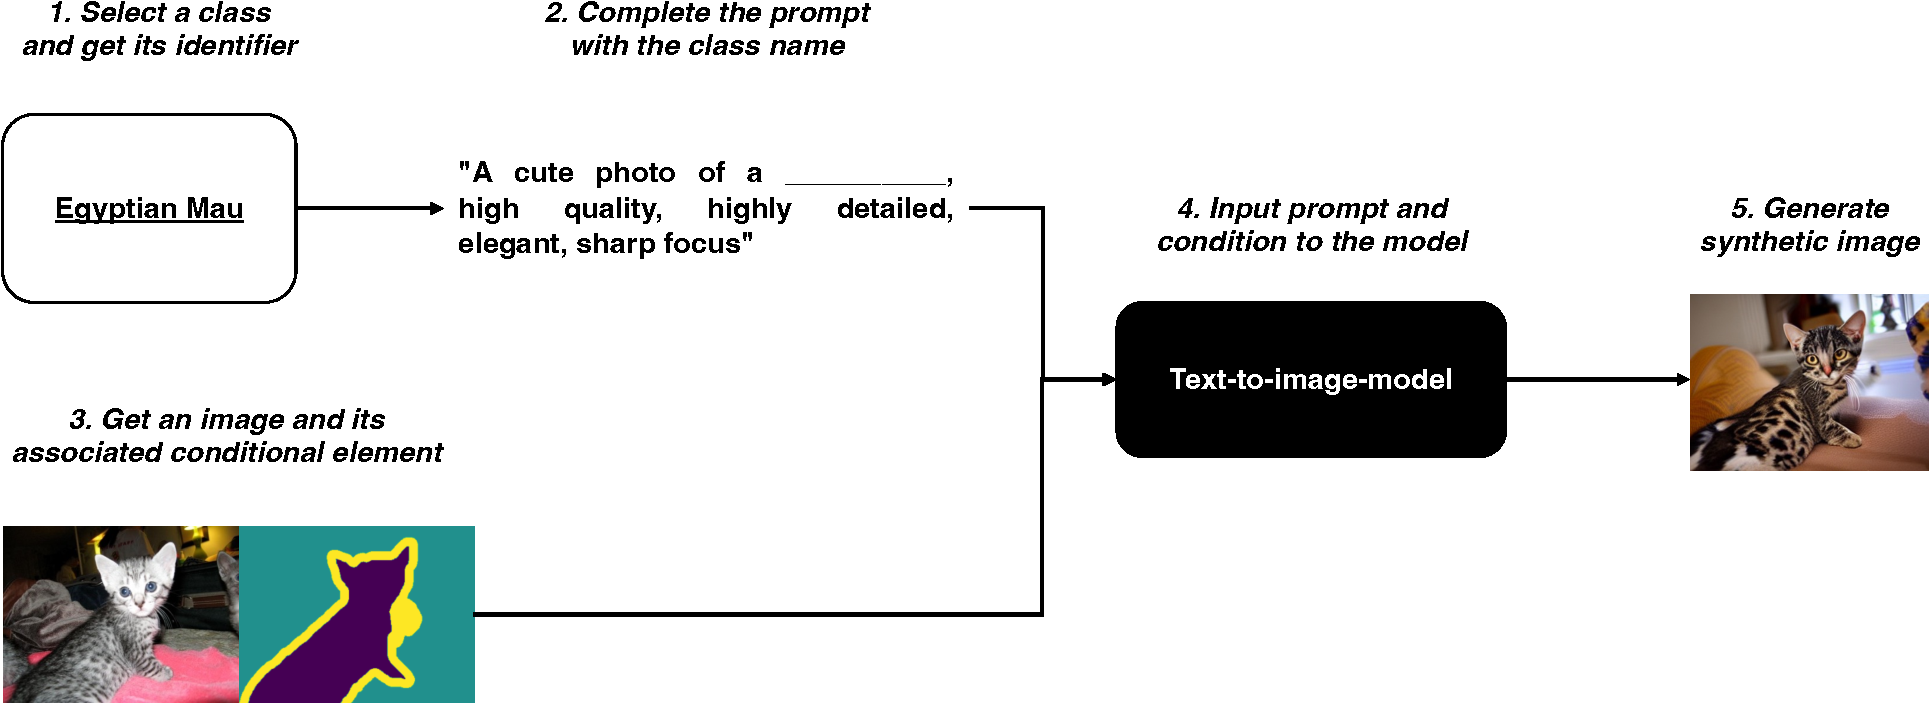
\includegraphics[width=1\textwidth]{Pictures/control-augmentation.pdf}
    \caption{\textbf{Augmentation schema using a conditionally controlled texto-to-image model}. The text-to-image model employs a conditional approach to generate an image based on a selected element.The idea is to extend class-name-based augmentation by conditional control. Thus, in this example, the generated image has as segmentation map the one given as condition. Consequently, it becomes feasible to augment a segmentation task by producing synthetic pairs of images and segmentation maps.}
    \label{fig:condaug}
\end{figure}